%
% main.tex -- Paper zum Thema <schwimmen>
%
% (c) 2020 Autor, OST Ostschweizer Fachhochschule
%
% !TEX root = ../../buch.tex
% !TEX encoding = UTF-8
%
\chapter{Die Optimale Flussüberquerung\label{chapter:schwimmen}}
\kopflinks{Thema}
\begin{refsection}
	\chapterauthor{Anna Pietak}
	
	
Das Überqueren eines Flusses ist seit jeher eine Herausforderung, die die Menschheit beschäftigt. Oft auch im Zusammenhang mit der Frage, wie man am besten mit einem Boot einen Fluss überquert, sind vielfältige Überlegungen angestellt worden. So hat sich auch Euler in seinem Werk \textit{De motu cymbarum remis propulsarum in fluviis} \cite{schwimmen:Euler_works} diese Frage gestellt. Einige einfache Ansätze könnten darin bestehen, den Fluss an einer flachen Stelle zu überqueren, wo man zu Fuss hindurch waten kann, oder ihn einfach gemütlich schwimmend zu durchqueren und einfach in kauf nehmen das die Strömung einen mitreisst.
	
	
Die zentrale Frage, die sich hier stellt, ist jedoch: Wie überquere ich einen Fluss am energieeffizientesten? In Abbildung \ref{fig:river_original} ist ein solcher Fluss dargestellt, der überquert werden soll.




\begin{figure}
    \centering
    \tikzset{every picture/.style={line width=0.75pt}} %set default line width to 0.75pt        

    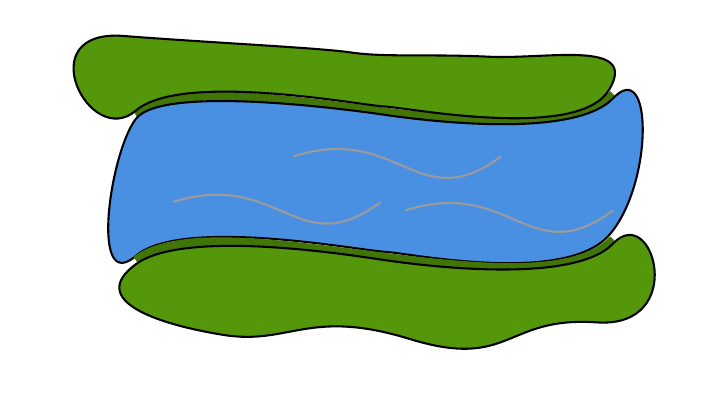
\begin{tikzpicture}[x=0.75pt,y=0.75pt,yscale=-1,xscale=1]
%uncomment if require: \path (0,300); %set diagram left start at 0, and has height of 300

%Curve Lines [id:da608977851192717] 
\draw [color={rgb, 255:red, 65; green, 117; blue, 5 }  ,draw opacity=1 ][line width=3]    (300,110) .. controls (340,80) and (493.51,138.06) .. (530,100) ;
%Shape: Polygon Curved [id:ds9392726871646548] 
\draw  [fill={rgb, 255:red, 74; green, 144; blue, 226 }  ,fill opacity=1 ] (300,112) .. controls (312.68,95.2) and (403.92,107.66) .. (420,110) .. controls (436.08,112.34) and (510.65,122.34) .. (530,102) .. controls (549.35,81.66) and (549.3,143.91) .. (528,168) .. controls (506.7,192.09) and (432.13,176.66) .. (420,176) .. controls (407.87,175.34) and (322.13,158.94) .. (300,178) .. controls (277.87,197.06) and (287.32,128.8) .. (300,112) -- cycle ;
%Curve Lines [id:da6433547723995421] 
\draw [color={rgb, 255:red, 65; green, 117; blue, 5 }  ,draw opacity=1 ][line width=3]    (300,180) .. controls (340,150) and (493.51,208.06) .. (530,170) ;
%Shape: Polygon Curved [id:ds34371397326569686] 
\draw  [fill={rgb, 255:red, 85; green, 151; blue, 11 }  ,fill opacity=1 ] (300,182) .. controls (323.56,164.66) and (403.92,177.66) .. (420,180) .. controls (436.08,182.34) and (510.65,192.34) .. (530,172) .. controls (549.35,151.66) and (566.44,213.06) .. (522,210) .. controls (477.56,206.94) and (481.01,233.06) .. (432,218) .. controls (382.99,202.94) and (374.13,221.23) .. (342,216) .. controls (309.87,210.77) and (276.44,199.34) .. (300,182) -- cycle ;
%Shape: Polygon Curved [id:ds3342416894164969] 
\draw  [fill={rgb, 255:red, 85; green, 151; blue, 11 }  ,fill opacity=1 ] (294,72) .. controls (339.58,75.49) and (387.92,77.66) .. (404,80) .. controls (420.08,82.34) and (442.15,80.63) .. (470,82) .. controls (497.85,83.37) and (542.72,73.49) .. (528,98) .. controls (513.28,122.51) and (432.13,106.66) .. (420,106) .. controls (407.87,105.34) and (322.13,88.94) .. (300,108) .. controls (277.87,127.06) and (248.42,68.51) .. (294,72) -- cycle ;
%Curve Lines [id:da7504908272245701] 
\draw [color={rgb, 255:red, 155; green, 155; blue, 155 }  ,draw opacity=1 ]   (318,152) .. controls (369.01,135.91) and (378,182) .. (418,152) ;
%Curve Lines [id:da01966435364089625] 
\draw [color={rgb, 255:red, 155; green, 155; blue, 155 }  ,draw opacity=1 ]   (376,130) .. controls (427.01,113.91) and (436,160) .. (476,130) ;
%Curve Lines [id:da5498107083025197] 
\draw [color={rgb, 255:red, 155; green, 155; blue, 155 }  ,draw opacity=1 ]   (430,156) .. controls (481.01,139.91) and (490,186) .. (530,156) ;




\end{tikzpicture}

    \caption{Fluss der überquert werden soll. Blau ist der Fluss eingezeichnet und grün das Ufer.}
    \label{fig:river_original}
\end{figure}

Für die Frage \textit{Wie schwimmt man am besten durch den Fluss?} wird zudem vorausgesetzt, dass das Ziel auf derselben Höhe auf der anderen Seite des Flusses erreicht werden soll. Was bedeutet das man die ganze Strömung durch flussaufwärs schwimmen kompensiert werden muss. Dies ist in Abbildung \ref{fig:river_points} veranschaulicht. Die Frage, die uns hier beschäftigt, lautet: Wie schwimmt man am besten von Punkt \(A\) nach Punkt \(B\)?






\begin{figure}
    \centering
       

    \tikzset{every picture/.style={line width=0.75pt}} %set default line width to 0.75pt        
    
    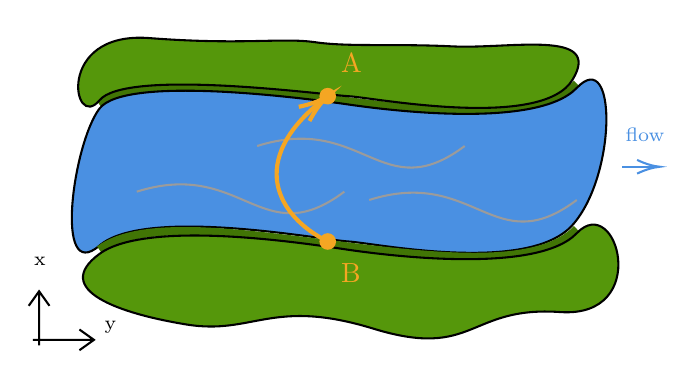
\begin{tikzpicture}[x=0.75pt,y=0.75pt,yscale=-1,xscale=1]
    %uncomment if require: \path (0,300); %set diagram left start at 0, and has height of 300
    
    %Curve Lines [id:da608977851192717] 
    \draw [color={rgb, 255:red, 65; green, 117; blue, 5 }  ,draw opacity=1 ][line width=3]    (300,110) .. controls (340,80) and (493.51,138.06) .. (530,100) ;
    %Shape: Polygon Curved [id:ds9392726871646548] 
    \draw  [fill={rgb, 255:red, 74; green, 144; blue, 226 }  ,fill opacity=1 ] (300,112) .. controls (312.68,95.2) and (403.92,107.66) .. (420,110) .. controls (436.08,112.34) and (510.65,122.34) .. (530,102) .. controls (549.35,81.66) and (549.3,143.91) .. (528,168) .. controls (506.7,192.09) and (432.13,176.66) .. (420,176) .. controls (407.87,175.34) and (322.13,158.94) .. (300,178) .. controls (277.87,197.06) and (287.32,128.8) .. (300,112) -- cycle ;
    %Curve Lines [id:da6433547723995421] 
    \draw [color={rgb, 255:red, 65; green, 117; blue, 5 }  ,draw opacity=1 ][line width=3]    (300,180) .. controls (340,150) and (493.51,208.06) .. (530,170) ;
    %Shape: Polygon Curved [id:ds34371397326569686] 
    \draw  [fill={rgb, 255:red, 85; green, 151; blue, 11 }  ,fill opacity=1 ] (300,182) .. controls (323.56,164.66) and (403.92,177.66) .. (420,180) .. controls (436.08,182.34) and (510.65,192.34) .. (530,172) .. controls (549.35,151.66) and (566.44,213.06) .. (522,210) .. controls (477.56,206.94) and (481.01,233.06) .. (432,218) .. controls (382.99,202.94) and (374.13,221.23) .. (342,216) .. controls (309.87,210.77) and (276.44,199.34) .. (300,182) -- cycle ;
    %Shape: Polygon Curved [id:ds3342416894164969] 
    \draw  [fill={rgb, 255:red, 85; green, 151; blue, 11 }  ,fill opacity=1 ] (324,78) .. controls (369.58,81.49) and (387.92,77.66) .. (404,80) .. controls (420.08,82.34) and (442.15,80.63) .. (470,82) .. controls (497.85,83.37) and (542.72,73.49) .. (528,98) .. controls (513.28,122.51) and (432.13,106.66) .. (420,106) .. controls (407.87,105.34) and (312.7,92.51) .. (300,108) .. controls (287.3,123.49) and (278.42,74.51) .. (324,78) -- cycle ;
    %Curve Lines [id:da7504908272245701] 
    \draw [color={rgb, 255:red, 155; green, 155; blue, 155 }  ,draw opacity=1 ]   (318,152) .. controls (369.01,135.91) and (378,182) .. (418,152) ;
    %Curve Lines [id:da01966435364089625] 
    \draw [color={rgb, 255:red, 155; green, 155; blue, 155 }  ,draw opacity=1 ]   (376,130) .. controls (427.01,113.91) and (436,160) .. (476,130) ;
    %Curve Lines [id:da5498107083025197] 
    \draw [color={rgb, 255:red, 155; green, 155; blue, 155 }  ,draw opacity=1 ]   (430,156) .. controls (481.01,139.91) and (490,186) .. (530,156) ;
    %Shape: Circle [id:dp01198373160385724] 
    \draw  [draw opacity=0][fill={rgb, 255:red, 245; green, 166; blue, 35 }  ,fill opacity=1 ] (406,106) .. controls (406,103.79) and (407.79,102) .. (410,102) .. controls (412.21,102) and (414,103.79) .. (414,106) .. controls (414,108.21) and (412.21,110) .. (410,110) .. controls (407.79,110) and (406,108.21) .. (406,106) -- cycle ;
    %Shape: Circle [id:dp6252725126232461] 
    \draw  [draw opacity=0][fill={rgb, 255:red, 245; green, 166; blue, 35 }  ,fill opacity=1 ] (406,176) .. controls (406,173.79) and (407.79,172) .. (410,172) .. controls (412.21,172) and (414,173.79) .. (414,176) .. controls (414,178.21) and (412.21,180) .. (410,180) .. controls (407.79,180) and (406,178.21) .. (406,176) -- cycle ;
    %Straight Lines [id:da006269855405936053] 
    \draw [color={rgb, 255:red, 74; green, 144; blue, 226 }  ,draw opacity=1 ]   (552,140) -- (568,140) ;
    \draw [shift={(570,140)}, rotate = 180] [color={rgb, 255:red, 74; green, 144; blue, 226 }  ,draw opacity=1 ][line width=0.75]    (10.93,-3.29) .. controls (6.95,-1.4) and (3.31,-0.3) .. (0,0) .. controls (3.31,0.3) and (6.95,1.4) .. (10.93,3.29)   ;
    %Shape: Axis 2D [id:dp579588107341299] 
    \draw  (268,223.4) -- (297.36,223.4)(270.94,200) -- (270.94,226) (290.36,218.4) -- (297.36,223.4) -- (290.36,228.4) (265.94,207) -- (270.94,200) -- (275.94,207)  ;
    %Curve Lines [id:da1687299064997403] 
    \draw [color={rgb, 255:red, 245; green, 166; blue, 35 }  ,draw opacity=1 ][line width=1.5]    (410,176) .. controls (385.7,163.93) and (370.61,137.1) .. (407.67,107.8) ;
    \draw [shift={(410,106)}, rotate = 143.13] [color={rgb, 255:red, 245; green, 166; blue, 35 }  ,draw opacity=1 ][line width=1.5]    (14.21,-4.28) .. controls (9.04,-1.82) and (4.3,-0.39) .. (0,0) .. controls (4.3,0.39) and (9.04,1.82) .. (14.21,4.28)   ;
    
    % Text Node
    \draw (415,84) node [anchor=north west][inner sep=0.75pt]  [color={rgb, 255:red, 245; green, 166; blue, 35 }  ,opacity=1 ] [align=left] {A};
    % Text Node
    \draw (415,185) node [anchor=north west][inner sep=0.75pt]  [color={rgb, 255:red, 245; green, 166; blue, 35 }  ,opacity=1 ] [align=left] {B};
    % Text Node
    \draw (552,120) node [anchor=north west][inner sep=0.75pt]  [color={rgb, 255:red, 74; green, 144; blue, 226 }  ,opacity=1 ] [align=left] {{\scriptsize flow}};
    % Text Node
    \draw (267,182) node [anchor=north west][inner sep=0.75pt]  [color={rgb, 255:red, 0; green, 0; blue, 0 }  ,opacity=1 ] [align=left] {{\scriptsize x}};
    % Text Node
    \draw (301,213) node [anchor=north west][inner sep=0.75pt]  [color={rgb, 255:red, 0; green, 0; blue, 0 }  ,opacity=1 ] [align=left] {{\scriptsize y}};
    
    
    \end{tikzpicture}
    

    \caption{Fluss der überquert werden soll. Blau ist der Fluss eingezeichnet und grün das Ufer. Die Strömung geht von liks nach rechts und ist mit dem Pfeil eingezeichnet. Unten links noch ein referenz kordinaten System.}
    \label{fig:river_points}
\end{figure}

In diesem Kapitel wird erläutert, wie man mittels des Variationsprinzips die optimale Schwimmroute über den Fluss findet so das man den geringsten Energieaufwand hat.


	
	
	
	
	% Ein paar Hinweise für die korrekte Formatierung des Textes
	% \begin{itemize}
		% \item
		% Absätze werden gebildet, indem man eine Leerzeile einfügt.
		% Die Verwendung von \verb+\\+ ist nur in Tabellen und Arrays gestattet.
		% \item
		% Die explizite Platzierung von Bildern ist nicht erlaubt, entsprechende
		% Optionen werden gelöscht. 
		% Verwenden Sie Labels und Verweise, um auf Bilder hinzuweisen.
		% \item
		% Beginnen Sie jeden Satz auf einer neuen Zeile. 
		% Damit ermöglichen Sie dem Versionsverwaltungssysteme, Änderungen
		% in verschiedenen Sätzen von verschiedenen Autoren ohne Konflikt 
		% anzuwenden.
		% \item 
		% Bilden Sie auch für Formeln kurze Zeilen, einerseits der besseren
		% Übersicht wegen, aber auch um GIT die Arbeit zu erleichtern.
		% \end{itemize}


%
% einleitung.tex -- Beispiel-File für die Einleitung
%
% (c) 2020 Prof Dr Andreas Müller, Hochschule Rapperswil
%
% !TEX root = ../../buch.tex
% !TEX encoding = UTF-8
%
\section{Herangehensweise\label{schwimmen:section:teil0}}
\rhead{Herangehensweise}

Es soll ermittelt werden, welche die energieeffizienteste Methode ist, um den Fluss zu überqueren. Da die Energie \(E\) mittels der Formel \[E = P \cdot t\] berechnet werden kann, wobei \(P\) für die Leistung und \(t\) für die Zeit steht, stellt sich heraus, dass die Energie für die Flussüberquerung direkt von der Zeit abhängt. Ergo sollte es möglich sein, nicht die Energie zu optimieren, sondern die Zeit.

Dies vereinfacht vieles, allerdings muss nun die Leistung, mit der geschwommen werden kann, begrenzt werden. Eine schwimmende Person kann nicht unbegrenzt schnell schwimmen und somit nicht in keiner Zeit am anderen Ufer ankommen.

\subsection{Variationsprinzip}
Das Variationsprinzip ist ein Konzept, das besagt, dass die Natur in vielen Fällen den optimalen Weg wählt. In diesem Fall ist es das Prinzip der kleinsten Wirkung, also des kleinsten Energieaufwand, der für die Flussüberquerung benötigt wird. Die Euler-Lagrange-Differentialgleichung ist das Werkzeug, um das Variationsprinzip zu berechnen. Das Lagrange-Integral gibt das Minimum der Wirkung zurück.



% Es soll ermitelt werden was die energieefizientiste Methode ist um den Fluss zu überqueren. Da die Energie \(E\) mittels der Formel \[E=P\cdot t\] berechnet werden kann wobei \(P\) für die Leistung und \(t\) für die Zeit steht, stehlt sich heraus das die Energie für die Flussüberquerung direkt von der Zeit abhängig ist. Ergo sollte es möglich sein nicht eine Optimierung der Energie sondern eine der Zeit zu machen. 
% Das vereinfacht vieles, jetzt muss man aber die Leistung mit der man schwimmen kann beschränken. Die schwimmende Person kann nicht unbeschränkt schnell schwimmen und dadurch in keiner Zeit am anderen Ufer ankommen.

% \subsection{Variationsprinzip}
% Das Variationsprinzip ist ein Konzept, das besagt, dass die Natur in vielen Fällen den optimalen Weg wählt. In diesem Fall ist es das Prinzip der kleinsten Wrikung, der kleinste Energieaufwand der für die Flussüberquerung gebraucht wird.
% Die Lagrange Formel ist das Werkzueg um das Variationsprinzip zu berechnen. Das Lagrange-Integral gibt das minimum der Wirkung zurück.









% Lorem ipsum dolor sit amet, consetetur sadipscing elitr, sed diam
% nonumy eirmod tempor invidunt ut labore et dolore magna aliquyam
% erat, sed diam voluptua \cite{schwimmen:bibtex}.
% At vero eos et accusam et justo duo dolores et ea rebum.
% Stet clita kasd gubergren, no sea takimata sanctus est Lorem ipsum
% dolor sit amet.

% Lorem ipsum dolor sit amet, consetetur sadipscing elitr, sed diam
% nonumy eirmod tempor invidunt ut labore et dolore magna aliquyam
% erat, sed diam voluptua.
% At vero eos et accusam et justo duo dolores et ea rebum.  Stet clita
% kasd gubergren, no sea takimata sanctus est Lorem ipsum dolor sit
% amet.



%
% teil1.tex -- Beispiel-File für das Paper
%
% (c) 2020 Prof Dr Andreas Müller, Hochschule Rapperswil
%
% !TEX root = ../../buch.tex
% !TEX encoding = UTF-8
%
\section{Herleitung
\label{schwimmen:section:naiver_weg}}
\rhead{Problemstellung}



% \begin{figure}
%     \centering
       
   

%     \tikzset{every picture/.style={line width=0.75pt}} %set default line width to 0.75pt        
    
%     \begin{tikzpicture}[x=0.75pt,y=0.75pt,yscale=-1,xscale=1]
% %uncomment if require: \path (0,300); %set diagram left start at 0, and has height of 300

% %Curve Lines [id:da608977851192717] 
% \draw [color={rgb, 255:red, 65; green, 117; blue, 5 }  ,draw opacity=1 ][line width=3]    (300,110) .. controls (340,80) and (493.51,138.06) .. (530,100) ;
% %Shape: Polygon Curved [id:ds9392726871646548] 
% \draw  [fill={rgb, 255:red, 74; green, 144; blue, 226 }  ,fill opacity=1 ] (300,112) .. controls (312.68,95.2) and (403.92,107.66) .. (420,110) .. controls (436.08,112.34) and (510.65,122.34) .. (530,102) .. controls (549.35,81.66) and (549.3,143.91) .. (528,168) .. controls (506.7,192.09) and (432.13,176.66) .. (420,176) .. controls (407.87,175.34) and (322.13,158.94) .. (300,178) .. controls (277.87,197.06) and (287.32,128.8) .. (300,112) -- cycle ;
% %Curve Lines [id:da6433547723995421] 
% \draw [color={rgb, 255:red, 65; green, 117; blue, 5 }  ,draw opacity=1 ][line width=3]    (300,180) .. controls (340,150) and (493.51,208.06) .. (530,170) ;
% %Shape: Polygon Curved [id:ds34371397326569686] 
% \draw  [fill={rgb, 255:red, 85; green, 151; blue, 11 }  ,fill opacity=1 ] (300,182) .. controls (323.56,164.66) and (403.92,177.66) .. (420,180) .. controls (436.08,182.34) and (510.65,192.34) .. (530,172) .. controls (549.35,151.66) and (566.44,213.06) .. (522,210) .. controls (477.56,206.94) and (481.01,233.06) .. (432,218) .. controls (382.99,202.94) and (374.13,221.23) .. (342,216) .. controls (309.87,210.77) and (276.44,199.34) .. (300,182) -- cycle ;
% %Shape: Polygon Curved [id:ds3342416894164969] 
% \draw  [fill={rgb, 255:red, 85; green, 151; blue, 11 }  ,fill opacity=1 ] (324,78) .. controls (369.58,81.49) and (387.92,77.66) .. (404,80) .. controls (420.08,82.34) and (442.15,80.63) .. (470,82) .. controls (497.85,83.37) and (542.72,73.49) .. (528,98) .. controls (513.28,122.51) and (432.13,106.66) .. (420,106) .. controls (407.87,105.34) and (312.7,92.51) .. (300,108) .. controls (287.3,123.49) and (278.42,74.51) .. (324,78) -- cycle ;
% %Curve Lines [id:da7504908272245701] 
% \draw [color={rgb, 255:red, 155; green, 155; blue, 155 }  ,draw opacity=1 ]   (318,152) .. controls (369.01,135.91) and (378,182) .. (418,152) ;
% %Curve Lines [id:da01966435364089625] 
% \draw [color={rgb, 255:red, 155; green, 155; blue, 155 }  ,draw opacity=1 ]   (376,130) .. controls (427.01,113.91) and (436,160) .. (476,130) ;
% %Curve Lines [id:da5498107083025197] 
% \draw [color={rgb, 255:red, 155; green, 155; blue, 155 }  ,draw opacity=1 ]   (430,156) .. controls (481.01,139.91) and (490,186) .. (530,156) ;
% %Shape: Circle [id:dp01198373160385724] 
% \draw  [draw opacity=0][fill={rgb, 255:red, 245; green, 166; blue, 35 }  ,fill opacity=1 ] (406,106) .. controls (406,103.79) and (407.79,102) .. (410,102) .. controls (412.21,102) and (414,103.79) .. (414,106) .. controls (414,108.21) and (412.21,110) .. (410,110) .. controls (407.79,110) and (406,108.21) .. (406,106) -- cycle ;
% %Shape: Circle [id:dp6252725126232461] 
% \draw  [draw opacity=0][fill={rgb, 255:red, 245; green, 166; blue, 35 }  ,fill opacity=1 ] (406,176) .. controls (406,173.79) and (407.79,172) .. (410,172) .. controls (412.21,172) and (414,173.79) .. (414,176) .. controls (414,178.21) and (412.21,180) .. (410,180) .. controls (407.79,180) and (406,178.21) .. (406,176) -- cycle ;
% %Straight Lines [id:da006269855405936053] 
% \draw [color={rgb, 255:red, 74; green, 144; blue, 226 }  ,draw opacity=1 ]   (552,140) -- (568,140) ;
% \draw [shift={(570,140)}, rotate = 180] [color={rgb, 255:red, 74; green, 144; blue, 226 }  ,draw opacity=1 ][line width=0.75]    (10.93,-3.29) .. controls (6.95,-1.4) and (3.31,-0.3) .. (0,0) .. controls (3.31,0.3) and (6.95,1.4) .. (10.93,3.29)   ;
% %Shape: Axis 2D [id:dp579588107341299] 
% \draw  (268,223.4) -- (297.36,223.4)(270.94,200) -- (270.94,226) (290.36,218.4) -- (297.36,223.4) -- (290.36,228.4) (265.94,207) -- (270.94,200) -- (275.94,207)  ;
% %Curve Lines [id:da1687299064997403] 
% \draw [color={rgb, 255:red, 245; green, 166; blue, 35 }  ,draw opacity=1 ][line width=1.5]    (410,176) .. controls (385.7,163.93) and (370.61,137.1) .. (407.67,107.8) ;
% \draw [shift={(410,106)}, rotate = 143.13] [color={rgb, 255:red, 245; green, 166; blue, 35 }  ,draw opacity=1 ][line width=1.5]    (14.21,-4.28) .. controls (9.04,-1.82) and (4.3,-0.39) .. (0,0) .. controls (4.3,0.39) and (9.04,1.82) .. (14.21,4.28)   ;
% %Straight Lines [id:da5117559499291524] 
% \draw [color={rgb, 255:red, 245; green, 166; blue, 35 }  ,draw opacity=1 ]   (386,146) -- (386,172) ;
% %Straight Lines [id:da7911427218260162] 
% \draw [color={rgb, 255:red, 245; green, 166; blue, 35 }  ,draw opacity=1 ]   (386,172) -- (404,172) ;
% %Shape: Axis 2D [id:dp020929963075495994] 
% \draw [color={rgb, 255:red, 144; green, 19; blue, 254 }  ,draw opacity=1 ] (414,164) -- (436,164)(416.2,146) -- (416.2,166) (429,159) -- (436,164) -- (429,169) (411.2,153) -- (416.2,146) -- (421.2,153)  ;
% %Straight Lines [id:da5963450198567739] 
% \draw [color={rgb, 255:red, 46; green, 0; blue, 255 }  ,draw opacity=1 ]   (480,148) -- (504,148) ;
% \draw [shift={(506,148)}, rotate = 180] [color={rgb, 255:red, 46; green, 0; blue, 255 }  ,draw opacity=1 ][line width=0.75]    (10.93,-3.29) .. controls (6.95,-1.4) and (3.31,-0.3) .. (0,0) .. controls (3.31,0.3) and (6.95,1.4) .. (10.93,3.29)   ;
% %Straight Lines [id:da016477493607424232] 
% \draw [color={rgb, 255:red, 46; green, 0; blue, 255 }  ,draw opacity=1 ]   (480,158) -- (498,158) ;
% \draw [shift={(500,158)}, rotate = 180] [color={rgb, 255:red, 46; green, 0; blue, 255 }  ,draw opacity=1 ][line width=0.75]    (10.93,-3.29) .. controls (6.95,-1.4) and (3.31,-0.3) .. (0,0) .. controls (3.31,0.3) and (6.95,1.4) .. (10.93,3.29)   ;
% %Straight Lines [id:da8245950958515168] 
% \draw [color={rgb, 255:red, 46; green, 0; blue, 255 }  ,draw opacity=1 ]   (480,138) -- (498,138) ;
% \draw [shift={(500,138)}, rotate = 180] [color={rgb, 255:red, 46; green, 0; blue, 255 }  ,draw opacity=1 ][line width=0.75]    (10.93,-3.29) .. controls (6.95,-1.4) and (3.31,-0.3) .. (0,0) .. controls (3.31,0.3) and (6.95,1.4) .. (10.93,3.29)   ;

% % Text Node
% \draw (415,84) node [anchor=north west][inner sep=0.75pt]  [color={rgb, 255:red, 245; green, 166; blue, 35 }  ,opacity=1 ] [align=left] {A};
% % Text Node
% \draw (415,185) node [anchor=north west][inner sep=0.75pt]  [color={rgb, 255:red, 245; green, 166; blue, 35 }  ,opacity=1 ] [align=left] {B};
% % Text Node
% \draw (552,120) node [anchor=north west][inner sep=0.75pt]  [color={rgb, 255:red, 74; green, 144; blue, 226 }  ,opacity=1 ] [align=left] {{\scriptsize flow}};
% % Text Node
% \draw (267,182) node [anchor=north west][inner sep=0.75pt]  [color={rgb, 255:red, 0; green, 0; blue, 0 }  ,opacity=1 ] [align=left] {{\scriptsize x}};
% % Text Node
% \draw (301,213) node [anchor=north west][inner sep=0.75pt]  [color={rgb, 255:red, 0; green, 0; blue, 0 }  ,opacity=1 ] [align=left] {{\scriptsize y}};
% % Text Node
% \draw (385,176.4) node [anchor=north west][inner sep=0.75pt]  [font=\scriptsize]  {$\textcolor[rgb]{0.96,0.65,0.14}{\Delta y}$};
% % Text Node
% \draw (367,158.4) node [anchor=north west][inner sep=0.75pt]  [font=\scriptsize]  {$\textcolor[rgb]{0.96,0.65,0.14}{\Delta x}$};
% % Text Node
% \draw (409,132.4) node [anchor=north west][inner sep=0.75pt]  [font=\scriptsize,color={rgb, 255:red, 144; green, 19; blue, 254 }  ,opacity=1 ]  {$\textcolor[rgb]{0.56,0.07,1}{c_{x}}$};
% % Text Node
% \draw (437,158.4) node [anchor=north west][inner sep=0.75pt]  [font=\scriptsize,color={rgb, 255:red, 144; green, 19; blue, 254 }  ,opacity=1 ]  {$\textcolor[rgb]{0.56,0.07,1}{c_{y}}$};
% % Text Node
% \draw (511,141.4) node [anchor=north west][inner sep=0.75pt]  [font=\scriptsize,color={rgb, 255:red, 144; green, 19; blue, 254 }  ,opacity=1 ]  {$\textcolor[rgb]{0.18,0,1}{u}$};


% \end{tikzpicture}



%     \caption{Fluss, der überquert werden soll. Die Strömungsgeschwindigkeit \(u\) ist dunkelblau eingezeichnet und bezieht sich auf die Geschwindigkeit des Flusses. Dabei ist zu beachten, dass diese nicht überall im Fluss gleich sein muss; sie könnte zum Ufer hin langsamer und in der Mitte des Flusses schneller sein. Somit ist sie von \(x\) abhängig. \(c_x\) und \(c_y\) bezeichnen die Geschwindigkeiten in \(x\)- und \(y\)-Richtung der schwimmenden Person. Diese geschwindigkeiten sind relative zu ruhigem wasser. Es ist definiert das die schwimmende Person in ruhigem Wasser mit einer Geschwindigkeit \(v\) schwimmen kann. Wobei sich \(c_x\) und \(c_y\) über die Formel \(v^2=c_x^2+c_y^2\) berechnen lässt. Diese Grössen beziehen sich daher auf ruhiges Wasser. \(\Delta x\) und \(\Delta y\) sind die sehr kleinen Distanzen auf der Strecke von \(A\) nach \(B\).
%     \label{fig:river_dif}}
% \end{figure}









% \begin{tikzpicture}[scale=1.5]

%     % Define coordinates and colors
%     \fill[blue!10] (0,0) rectangle (2,5);  % Blue rectangle
%     \draw[->] (-0.5,0) -- (2.5,0) node[right] {$x$};  % x-axis
%     \draw[->] (0,-0.5) -- (0,5.5) node[above] {$y$};  % y-axis

%     % Draw the curve
%     \draw[thick,red] plot[domain=0:2, samples=100] (\x,{(\x)^2}) node[right] {$(a, A)$};

%     % Plot points
%     \filldraw[black] (0,0) circle (1.5pt) node[below left] {$(0,0)$};
%     \filldraw[black] (2,4) circle (1.5pt) node[below right] {$(a,A)$};

%     % Draw vertical arrows representing v(x)
%     \foreach \x in {0,0.4,0.8,1.2,1.6,2} {
%         \draw[->] (\x,4.5) -- (\x,5);
%     }

%     % Arrow on the curve
%     \draw[red,->] (1,1) -- (1.5,2.25);

%     % Light background for the rectangle
%     % \draw[blue!20, fill=blue!20] (0,0) rectangle (2,5);

% \end{tikzpicture}





Hier ist eine Schritt für Schritt Darstellung der Herleitung zur optimalen Flussüberquerung dargestellt. 

\begin{figure}
    \centering
        \centering
        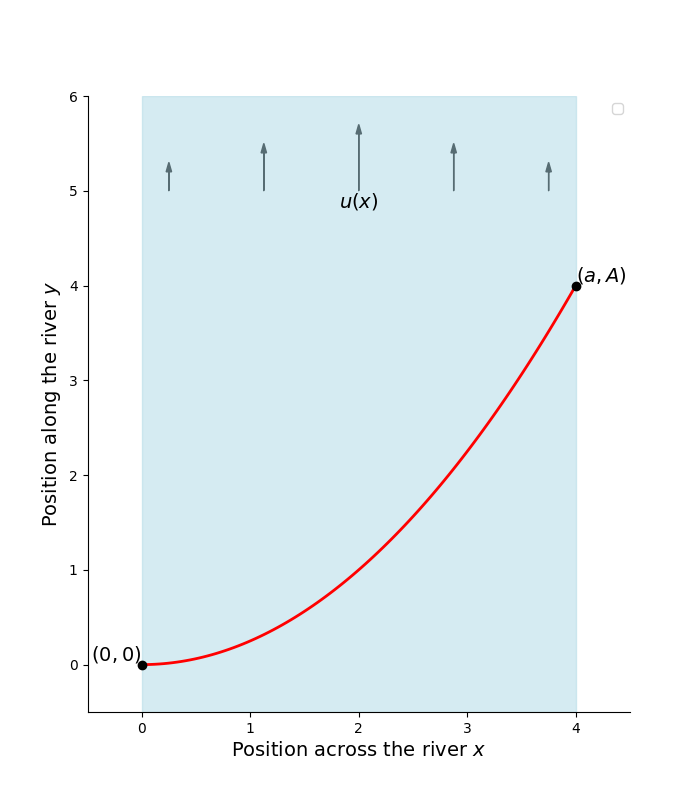
\includegraphics[width=0.6\textwidth]{papers/schwimmen/Grafiken/Figure_1.png}	
        \caption{Stillstehender Fluss}
        \label{fig:river_template}
\end{figure}

Ziel ist es die schnellste Rute über den Fluss zu finden. In Abbildung \ref{fig:river_template} ist dies abgebildet, wobei \(a\) die Flussbreite ist und \(A\) die Distanz dem Fluss entlang. In diesem Fall ist \(A=0\) da man am andern Ufer auf gleicher Höhe ankommt.

\subsubsection{Wichtige Kenngrössen}
Ein paar wichtige Kenngrössen für die Herleitung sind in Tabelle \ref{table:Wichtige_Kenngroessen} zufinden.

\begin{table}
    \centering
    \renewcommand{\arraystretch}{1.3}
    \begin{tabularx}{\textwidth}{@{}ll>{\raggedright\arraybackslash}p{7cm}@{}}
        \multicolumn{3}{c}{Wichtige Grössen} \\
        % \specialrule{.1em}{.05em}{.05em}
        % \textbf{Dataset} & \textbf{\(\mu\) in \(\mathrm{ps}\)} & \textbf{\(\sigma\) in \(\mathrm{ps}\)} \\
        \hline
        \(a\)   &   Flussbreite  &   definiert von der Umgebung \\
        \(c\)   &   Schwimmgeschwindigkeit        &   Definiert von der schwimmenden Person       \\
        \(v(x)\)   &   Flussgeschwindigkeit         &   Ist von der \(x\)-Position im Fluss abhängig     \\
        \((0,0)\)   &   Startpunkt         &   Startpunkt am Flussufer     \\
        \((a,A)\)   &   Endpunkt         &   Endpunkt auf anderer Uferseite aber auf gleicher Höhe     \\
        \specialrule{.1em}{.05em}{.05em}
    \end{tabularx}
    \caption{Wichtige Kenngrössen für die Herleitung}
    \label{table:Wichtige_Kenngroessen}
\end{table}


\subsubsection{Schwimmgeschwindigkeiten}

Als erstes werden die Geschwindigkeiten der Schwimmenden Person definiert. Mittels den Schwimmrichtungsvektoren und dem Flussvektor, können folgende Geschwindigkeiten für die in \(x\)- und \(y\)-Richtungen geschwommenen Geschwindigkeiten relativ zum Ufer genommen werden:
\begin{align}
    c_x &= c\cdot cos(\theta) \label{eq:c_x_equation}\\
    c_y &= u(x) + c \cdot sin(\theta) \label{eq:c_y_equation}
\end{align}

\(c_x\) ist die Geschwindigkeit in \(x\)-Richtung der schwimmenden Person, \(c_y\) ist die Geschwindigkeit in \(y\)-Richtung wie auch die Flussgeschwindigkeit. Dabei ist der Winkel \(\theta\) der Schwimmwinkel in Bezug auf die \(x\)-Richtung.


\subsubsection{Zeitoptimierung}

Da für den geringsten Energiekonsum die Zeit optimiert wird, hier das Integral für die total gebrauchte Zeit der Flussüberquerung:
\begin{equation}
    T = \int_0^adt \label{eq:Time_river_1}
\end{equation}
Da \(dt = \frac{dx}{c_x}\), die Zeit die es benötigt um sich ein kleines Stück in \(x\)-Richtung zu bewegen, von der Geschwindigkeit in \(x\)-Richtung abhängt, kann man \ref{eq:Time_river_1} erweitern zu

\begin{equation}
    T = \int_0^adt = \int_0^a\frac{dx}{||c_x||} = \int_0^a\frac{dx}{c\cdot cos(\theta)} \label{eq:Time_river_2}.
\end{equation}

Wobei \(||c_x||\) den Vektor \(c_x\) definiert. 


\subsubsection{Beziehung der \(x\)- und \(y\)-Geschwindigkeiten}

Als nächstes die Beziehung der \(x\)- und \(y\)-Geschwindigkeiten im System. Dies ist auch am Schluss wichtig um den genauen Schwimmverlauf der schwimmenden Person observieren zu können.

Die \(y\)-Geschwindigkeit soll im Bezug zur \(x\)-Richtung gegeben werden. Die Schwimmgeschwindigkeit in \(y\)-Richtung is gegeben durch
\begin{equation}
    c_y = \frac{dy}{dt}
\end{equation}
worauf die Kettenregel angewendet werden kann um
\begin{equation}
    \frac{dy}{dt} = \frac{dy}{dx} = \frac{dx}{dt} = \frac{dy}{dx}\cdot c_x = \frac{dy}{dx}\cdot c\cdot cos(\theta)
\end{equation}
zubekommen. Mittels \(c_y = u(x) + c\cdot sin(\theta)\) bekommt man die Beziehung der \(x\)- und \(y\)-Geschwindigkeiten:
\begin{equation}
    \frac{dy}{dx} = \frac{u(x) + c \cdot sin(\theta)}{c \cdot sin(\theta)} \label{eq:dy_dx}
\end{equation}



\subsubsection{Auflösen nach \(\theta\)}

Der letzte Schritt für das aufstellen des Integrals ist es eine Formel für den Winkel \(\theta\) zu haben.
Ausgehend von \ref{eq:dy_dx} können Umformungen gemacht werden
\begin{align}
    \frac{dy}{dx} &= \frac{\dot{y}}{\dot{x}} = \frac{c_y}{c_x} = \frac{u(x) + c \cdot sin(\theta)}{c \cdot sin(\theta)} \\
    \frac{dy}{dx} &= \frac{u}{c}\cdot sec(\theta) + tan(\theta) \\
    \frac{dy}{dx} &= \frac{u}{c}\cdot sec(\theta) + \sqrt{sec^2(\theta)-1} \\
\end{align}

es sein folgende Formeln für die Umformungen zu beachten: \(\frac{1}{cos(\theta)} = sec(\theta)\) und \(sec^2(\theta)-tan^2(\theta) = 1\). Durch Quartieren und \(\frac{dy}{dx} = y'\) folgt 
\begin{equation}
    (\frac{u^2}{c^2}-1)\cdot sec^2(\theta) - \frac{2uy'}{c}\cdot sec(\theta) + y'^2 +1 = 0
\end{equation}
als Gleichung. Durch die Mitternachtsformel bekommt man 
\begin{equation}
    sec(\theta) = \frac{\frac{2uy'}{c} \pm \sqrt{4(y'^2-\frac{u^2}{c^2} + 1)}}{2(\frac{u^2}{c^2}-1)}
\end{equation}
für den Winkel \(\theta\). Durch weiteres Umformen bekommt man:
\begin{equation}
    \frac{1}{c}\cdot sec(\theta) = \frac{-uy' \mp \sqrt{c^2(y'^2+1)-u^2}}{c^2-u^2} \label{eq:theta_1}
\end{equation}


\subsubsection{Zeit Integral}

Nun kann man die Formel \ref{eq:theta_1} für den Winkel, in das Zeit-Integral einfügen:

\begin{equation}
    T = \int_0^adt = \int_0^a\frac{dx}{c\cdot cos(\theta)} = \int_0^a \frac{-uy' \mp \sqrt{c^2(y'^2+1)-u^2}}{c^2-u^2} dx
    \label{eq:Time_river_2} 
\end{equation}

Dieses Integral  beschreibt die Zeit die für die Flussüberquerung benötigt wird. 



\subsubsection{Lagrange-Funktion} 
Um die Rute zu finden die die kürzeste Zeit für die Flussüberquerung benötigt wendet man das Variationsprinzip. Für das braucht man das sogenannte Lagrange-Integral welches minimiert werden soll in diesem Fall \ref{eq:Time_river_2}. 
Aus dem Lagrange-Integral \ref{eq:Time_river_2} kann die Lagrange-Funktion
\begin{equation}\label{eq:lagrange_integral}
    L(x, y, y') = \frac{-uy' \mp \sqrt{c^2(y'^2+1)-u^2}}{c^2-u^2}
\end{equation}
herausgelesen werden. 

\subsubsection{Euler-Lagrange-Differentialgleichung} Die Euler-Lagrange-Differentialgleichung kann vereinfacht werden, da sie nicht direkt von \(y\) abhängig ist:

\begin{align}
    \frac{\partial L}{\partial y} - \frac{d}{dx}\frac{\partial L}{\partial y'} = 0 - \frac{d}{dx}\frac{\partial L}{\partial y'} &= 0 \\
    \frac{d}{dx}\frac{\partial L}{\partial y'} &= 0.
\end{align}

Daraus folgt die Ableitung der Lagrange-Funktion:
\begin{align}
    \frac{\partial L}{\partial y'} &= \text{constant} \label{eq:Lagrange_derivites_1}\\
    \frac{\partial L}{\partial y'} &= \frac{\partial}{\partial y'} \biggl (\frac{-uy' \mp \sqrt{c^2(y'^2+1)-u^2}}{c^2-u^2}\biggr) \\
    &= \frac{c^2\cdot y'}{\sqrt{c^2(y'^2-u^2)}(c^2-u^2)} - \frac{u}{c^2-u^2} \\
    &=  \frac{1}{c^2-u^2} \biggl( \frac{c^2\cdot y'}{\sqrt{c^2(y'^2-u^2)}} - u \biggr ) \\
    &= \text{constant} = \frac{1}{g}.\label{eq:Lagrange_derivites_2}
\end{align}
Auflösung nach \(y'\):
   
\begin{equation}
    y' = \frac{c^2 + g\cdot u - u^2}{c \cdot \sqrt{u^2-2\cdot g\cdot u - c^2 + g^2}} \label{eq:angle} \\
\end{equation}

\(y'\) gibt an mit welchem Verhältnis von \(y\) zu \(x\) sich die Schwimmende Person im Wasser bewegt.
































% \subsubsection{Zeitoptimierung} Die Zeit \(T\), die für die Flussüberquerung benötigt wird, kann mittels
% \[
% T = \int \frac{1}{v} \, ds
% \]
% berechnet werden, wobei \(v\) die Geschwindigkeit ist und \(s\) die dabei zurückgelegte Strecke.

% \subsubsection{Zeit für ein Streckenstück} Die Zeit, die für ein sehr kleines Streckenstück entlang der Schwimmroute benötigt wird, kann ermittelt werden, indem man diese kleine Strecke durch die Geschwindigkeit auf dieser kleinen Strecke teilt. Dies sieht so aus:
% \begin{equation}\label{eq:time_for_distance_pice}
%     \frac{ds}{\sqrt{(c_y - u)^2 + c_x^2}},
% \end{equation}
% wobei \(u\) die Geschwindigkeit des Flusses bzw. der Strömung an dieser Stelle im Fluss ist. \(c_x\) und \(c_y\) bezeichnen die Geschwindigkeiten der schwimmenden Person in \(x\)- und \(y\)-Richtung, relativ zum Ufer. Die korrektur mit \(u\) dient der Kompenation der Strömung. Eine grafische Darstellung ist in Abbildung \ref{fig:river_dif} zu sehen.

% \subsubsection{Zeit für die Strömungskompensation} Die Zeit, die zusätzlich zur Flussüberquerung benötigt wird, um die Strömung zu kompensieren, ist definiert als 
% \begin{equation}\label{eq:time_compenation}
%     \frac{dx}{u}.
% \end{equation}

% \subsubsection{Gesamte Zeit} Die gesamte Zeit für ein sehr kleines Streckenstück kann mittels der Gleichungen \eqref{eq:time_for_distance_pice} und \eqref{eq:time_compenation} hergeleitet werden. Es folgt für die Zeit eines Wagestücks
% \begin{equation}\label{eq:time_pice_total}
%     dt = \frac{dx}{u} + \frac{ds}{\sqrt{(c_y - u)^2 + c_x^2}}.
% \end{equation}

% \subsubsection{Strecke}
% Für allgemeine Fälle kann die Distanz einer Strecke mit der Formel
% \[
% ds = \sqrt{\Delta x^2 + \Delta y^2} \approx \sqrt{1 + y'^2} \, dx
% \]
% angenähert werden, wobei sich die Variablen wieder auf Abbildung \ref{fig:river_dif} beziehen.

% \subsubsection{Integral} Nun ist es an der Zeit, ein Integral für die Zeit, die benötigt wird, um den Fluss zu überqueren, aufzustellen, basierend auf den obigen Formeln. Das Integral wird entlang \(x\), also vom einten Ufer \(A\) zum anderen Ufer \(B\), des Flusses, entlang Integriert. Das Integral
% \begin{equation}\label{eq:integral_time}
%     T = \int_A^B L(x, y, y') \, dx = \int_A^B \biggl( \frac{1}{u} + \frac{\sqrt{1 + y'^2}}{\sqrt{(c_y - u)^2 + c_x^2}} \biggr) dx
% \end{equation}
% soll für eine möglichst kleine Zeit \(T\) optimiert werden, um die energieeffizienteste Überquerung zu erreichen. Es ist zu beachten das \(u\), \(c_x\), \(c_y\) sowohl als auch \(y'\) von x abhängig sind, bzw. sie sind alle von der aktuellen Position im Fluss abhängig. Somit müssten sie eigentlich \(u(x)\), \(c_x(x)\), \(c_y(x)\) sowohl als auch \(y'(x)\) heisen, der Einfachheitshalber werden sie aber nur in der verkürzten Schreibweise geschrieben.

% \subsubsection{Lagrange-Funktion} Aus dem Lagrange-Integral \ref{eq:integral_time} kann die Lagrange-Funktion
% \begin{equation}\label{eq:lagrange_integral}
%     L(x, y, y') = \frac{1}{u} + \frac{\sqrt{1 + y'^2}}{\sqrt{(c_y - u)^2 + c_x^2}}
% \end{equation}
% herausgelesen werden. Die Lagrange-Funktion wird für das Variationsprinzip benötigt, um die Funktion für die energieeffizienteste Methode für die Flussüberquerung zu berechnen. Wobei \(y'\) angibt wie schnell sich die schwimmende Person in y-Richtung bewegt während sie sich in x-Richtung bewegt.

% \subsubsection{Euler-Lagrange-Differentialgleichung} Die Euler-Lagrange-Differentialgleichung kann vereinfacht werden, da sie nicht direkt von \(y\) abhängig ist:

% \begin{align}
%     \frac{\partial L}{\partial y} - \frac{d}{dx}\frac{\partial L}{\partial y'} = 0 - \frac{d}{dx}\frac{\partial L}{\partial y'} &= 0 \\
%     \frac{d}{dx}\frac{\partial L}{\partial y'} &= 0.
% \end{align}

% Daraus folgt die Ableitung der Lagrange-Funktion:
% \begin{align}
%     \frac{\partial L}{\partial y'} &= \text{constant} \label{eq:Lagrange_derivites_1}\\
%     \frac{\partial L}{\partial y'} &= \frac{\partial}{\partial y'} \biggl( \frac{1}{u} + \frac{\sqrt{1 + y'^2}}{\sqrt{(c_y - u)^2 + c_x^2}} \biggr) \\
%     &= \frac{1}{\sqrt{(c_y - u)^2 + c_x^2}} \cdot \frac{y'}{\sqrt{1 + y'^2}}\\
%     &= \text{constant} = \frac{1}{g}.\label{eq:Lagrange_derivites_2}
% \end{align}
% Auflösung nach \(y'\):
% \begin{align}
%     y' &= \sqrt{(c_y - u)^2 + c_x^2} \cdot \sqrt{1 + y'^2} \cdot \frac{1}{g} \\
%     y' &= \sqrt{\frac{c_y^2 - 2 \cdot c_y \cdot u + u^2 + c_x^2}{g^2 - c_y^2 + 2 \cdot c_y \cdot u - u^2 - c_x^2}}.\label{eq:angle}
% \end{align}

% \(y'\) gibt an wie schnell sich die schwimmende Person in y-Richtung während sie sich in x-Richtung bewegt, um das andere Ufer am Effizientesten zu erreichen.


% Wird das Integral über \(y'\) gebildet, erhält man die Zeit:
% \begin{equation}\label{eq:time_integral}
%     T = y = \int \sqrt{\frac{c_y^2 - 2 \cdot c_y \cdot u + u^2 + c_x^2}{g^2 - c_y^2 + 2 \cdot c_y \cdot u - u^2 - c_x^2}} \, dx
% \end{equation}





















        

%     \caption{Fluss der überquert werden soll. Die Strömungsgeschwindigkeit \(u\) dunkelblau eingezeichnet beziht sich auf die geschwindigkeit des Flusses, dabei ist zu beachten das diese nicht überal im Fluss gleich sein muss, sie könnte zum Ufer des Flusses hin langamer sein und in der mitte des Flusses schneller. Somit ist sie von \(x\) abhängig. \(c_x\)} und \(c_y\) bezeichenen die Geschwindigkeiten in \(x\)- und \(y\)-Richtung der schwimmenden Person. \(\Delta x\) und \(\Delta y\) sind die sehr kleinen Distanzen auf der Strecke von A nach B.
%     \label{fig:river_dif}
% \end{figure}


% \textbf{Zeitoptimierung} Die Zeit \(T\) die Für die Flussüberquerung gebraucht wird kann mittels \[T=\int{\frac{1}{v}ds}\] berechnet werden, wobei \(v\) die Geschwindigkeit ist und \(s\) die dabei zurückgelegte Strecke. 

% \textbf{Zeit für ein Streckenstück} Die Zeit die für ein sehr kleines streckenstück benötigt wird kann ermittelt werden in dem man diese kleine Strecke durch die Geschwindigkeit auf dieser kleinen strecke teilt. Dies sith so aus:
% \begin{equation}\label{eq:time_for_distance_pice}
%     \frac{ds}{\sqrt{(c_y-u)^2+c_x^2}}
% \end{equation}
% Wobei \(u\) die geschwindigkeit des Flsses bzw. der Strömung and dieser Stelle im Fluss ist. \(c_x\) und \(c_y\) bezeichen die Geschwindigkeiten der schwimmenden Person in Axenrichtung in \(x\) und \(y\) richtung, eine Graphische darstellung ist in Abbildung \ref{fig:river_dif} dargestellt.

% \textbf{Zeit für die Strömungskompensation} Die Zeit die zusätzlich zur Flussüberquerung bebraucht wird um die Strömung zu kompensieren ist definiert als 
% \begin{equation}\label{eq:time_compenation}
%     \frac{dx}{u}
% \end{equation}

% \textbf{Gesamte Zeit} Die gesmate Teit für ein sehr kleines Streckenstück kann mitels den Gleicungen \ref{eq:time_for_distance_pice} und \ref{eq:time_compenation} hergeleitet werden, es folgt: 
% \begin{equation}\label{eq:time_pice_total}
%     \frac{dx}{u} + \frac{ds}{\sqrt{(c_y-u)^2+c_x^2}}.
% \end{equation}


% \textbf{Strecke}
% Für allgemeine Fälle kann die Distanz einer Strecke mit der Formel
% \begin{equation}
%     ds=\sqrt{\Delta x^2 + \Delta y^2} \approx \sqrt{1+y'^2}dx
% \end{equation}
% angenähert werden, wobei sich die Variabeln wider auf Abbildung \ref{fig:river_dif} bezihn. 

% \textbf{Integral} Nun ist es so weit das ein Integral für die Zeit die gebraucht wird um den Fluss zu überqueren aufgestellt werden kann, mit den Formeln von oben. Das Integral:
% \begin{equation}\label{eq:integral_time}
%     T=\int L(x,y,y')dx = \int\frac{1}{u} + \frac{\sqrt{1+y'^2}}{\sqrt{(c_y-u)^2+c_x^2}}dx
% \end{equation}
% soll für eine möglischst kleine Zeit \(T\) optimiert werden um die energieefizientiste überquerung zu bekommen

% \textbf{Lagrange-Funktion} Aus dem Langrange-Integral \ref{eq:integral_time} kann die Lagrange Funktion 
% \begin{equation}\label{eq:lagrange_integral}
%     L(x,y,y')dx = \frac{1}{u} + \frac{\sqrt{1+y'^2}}{\sqrt{(c_y-u)^2+c_x^2}}dx
% \end{equation}
% herausgelesen werden. Die Lagrange-Funtion wird für das Variationsprinzip gebraucht um die Funktion für die Energieefizäntiste Methode für die Flussüberquerung zu berechnen.


% \textbf{Euler-Lagrange Formel} Euler-Lagrange Formel kann vereinfacht werden da sie nicht direkt von \(y\) abhägig ist. Ableitungen von der Lagrange-Funktion:
% \begin{equation}\label{eq:Lagrange_derivites_1}
%     \frac{\partial L}{\partial y'}=constant
% \end{equation}
% \begin{multline}\label{eq:Lagrange_derivites_2}
%     \frac{\partial L}{\partial y'}=\frac{\partial}{\partial y'}\frac{1}{u}+\frac{\sqrt{1+y'^2}}{\sqrt{(c_y-u)^2+c_x^2}}\\
%     =\frac{1}{\sqrt{(c_y-u)^2+c_x^2}}\frac{y'}{\sqrt{1+y'^2}}=constant=\frac{1}{g}
% \end{multline}\label{eq:Lagrange_derivites_y'}
% nach \(y'\) auflössen
% \begin{align}
%     y'&=\sqrt{(c_y-u)^2+c_x^2}\cdot\sqrt{1+y'^2}\cdot\frac{1}{g} \\
%     y'&=\sqrt{\frac{c_y^2-2\cdot c_y\cdot u+u^2+c_x^2}{g^2-c_y^2+2\cdot c_y\cdot u-u^2-c_x^2}}\label{eq:angle}
% \end{align}
% Bildet man das Integral um \(y'\) bekommt man die Zeit
% \begin{equation}\label{eq:time_integral}
%     T=y=\int\sqrt{\frac{c_y^2-2\cdot c_y\cdot u+u^2+c_x^2}{g^2-c_y^2+2\cdot c_y\cdot u-u^2-c_x^2}}dx
% \end{equation}






%
% 03_auswertung.tex -- Beispiel-File für teil2 
%
% (c) 2020 Prof Dr Andreas Müller, Hochschule Rapperswil
%
% !TEX root = ../../buch.tex
% !TEX encoding = UTF-8
%
\section{Visuelle Darstellung der Flussüberquerung
\label{schwimmen:section:bildliche_darstellung}}
\kopfrechts{Visuelle Darstellung der Flussüberquerung}
\begin{figure}
    \centering
    \begin{subfigure}{0.48\textwidth}
        \centering
        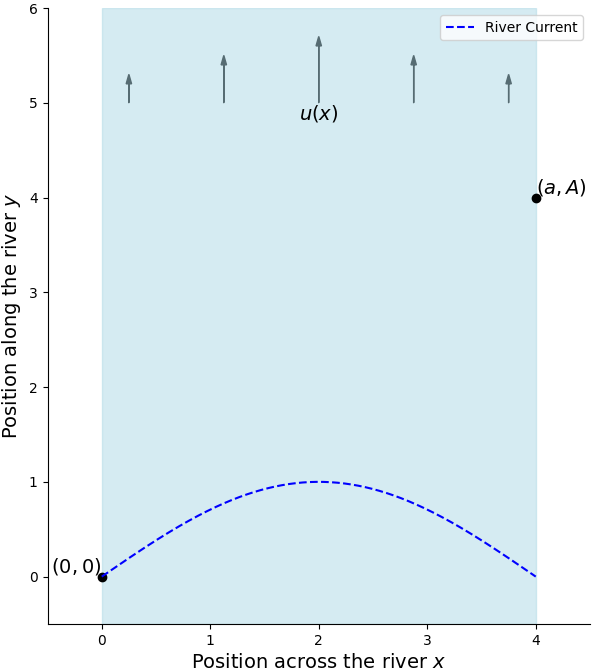
\includegraphics[width=\textwidth]{papers/schwimmen/Grafiken/Figure_2-crop.png}	
        \caption{Flussströmung}
        \label{fig:no_velocity}
    \end{subfigure}
    \hfill  
    \begin{subfigure}{0.48\textwidth}
        \centering
        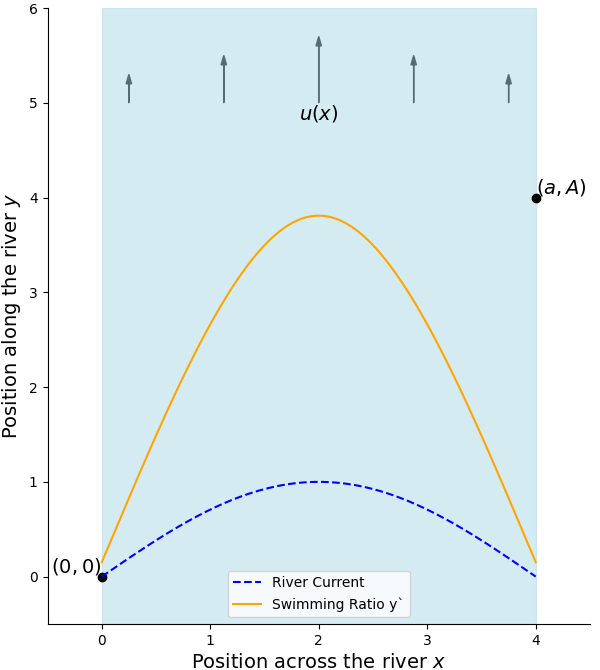
\includegraphics[width=\textwidth]{papers/schwimmen/Grafiken/Figure_3-crop.png}	
        \caption{\(y' = \frac{dy}{dx}\)}
        \label{fig:diagonal_velocity}
    \end{subfigure}
    \par\bigskip
    \begin{subfigure}{0.48\textwidth}
        \centering
        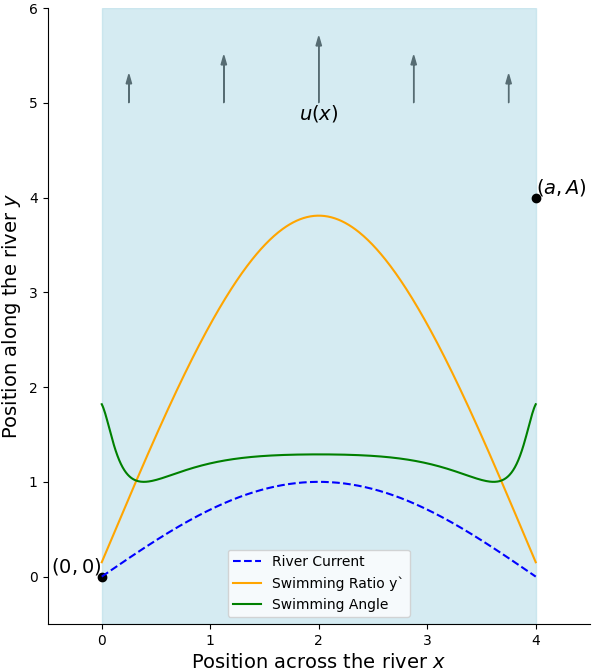
\includegraphics[width=\textwidth]{papers/schwimmen/Grafiken/Figure_4-crop.png}	
        \caption{Winkel der Schwimmenden Person}
        \label{fig:squerd_velocity}
    \end{subfigure}
    \hfill  
    \begin{subfigure}{0.48\textwidth}
        \centering
        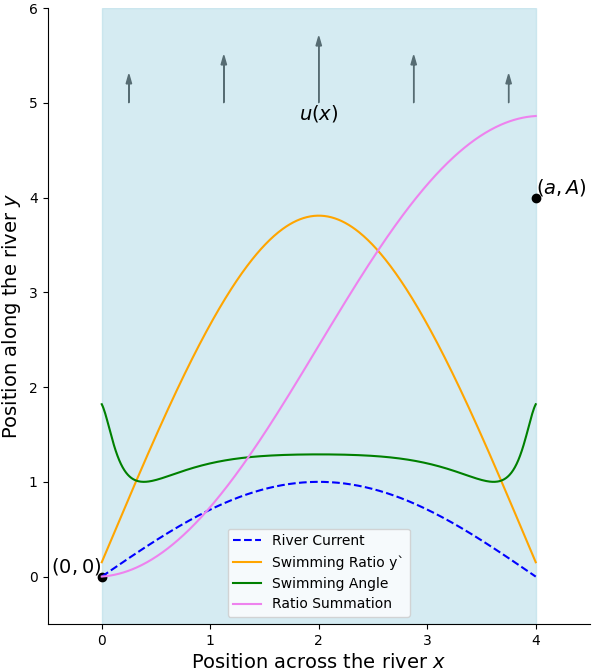
\includegraphics[width=\textwidth]{papers/schwimmen/Grafiken/Figure_5-crop.png}	
        \caption{Aufsumierte Steigung}
        \label{fig:sin_velocity}
    \end{subfigure}
    \par\bigskip
    \caption{Die vier Grafiken stellen verschiedene Graphen dar die für die Flussüerquerung zentrall sind, (a) stellt die Flussströmung dar, (b) das Verhältis zwischen was in \(x\)- und \(y\)-Richtung geschwommen wird, (c) den Winkel der aus dem Verhältnis folgt und (d) das aufsummierte Verhältnis}
    \label{fig:river_pfrofiles}
\end{figure}
%
% papers/schwimmen/


Die Gleichung \eqref{eq:angle} beschreibt das Verhältnis \(\frac{dy}{dx}\)
für die Schwimmrichtung der schwimmenden Person, um die optimale
Flussüberquerung zu erreichen.

In Abbildung \ref{fig:river_pfrofiles} ist eine visuelle Darstellung
für die Flussüberquerung. Es ist zu sehen, dass die Person am
Uferrand weit nach oben schwimmt und dann in der Mitte des Flusses
fast keine Änderung in \(y\)-Richtung macht sondern nur in
\(x\)-Richtung. Sie versucht also, den Bereich stärkerer Strömung,
in der Mitte des Flusses, möglichst schnell hinter sich zu bringen.




% %
% teil3.tex -- Beispiel-File für Teil 3
%
% (c) 2020 Prof Dr Andreas Müller, Hochschule Rapperswil
%
% !TEX root = ../../buch.tex
% !TEX encoding = UTF-8
%
\section{Teil 3
\label{000template:section:teil3}}
\rhead{Teil 3}
Sed ut perspiciatis unde omnis iste natus error sit voluptatem
accusantium doloremque laudantium, totam rem aperiam, eaque ipsa
quae ab illo inventore veritatis et quasi architecto beatae vitae
dicta sunt explicabo. Nemo enim ipsam voluptatem quia voluptas sit
aspernatur aut odit aut fugit, sed quia consequuntur magni dolores
eos qui ratione voluptatem sequi nesciunt. Neque porro quisquam
est, qui dolorem ipsum quia dolor sit amet, consectetur, adipisci
velit, sed quia non numquam eius modi tempora incidunt ut labore
et dolore magnam aliquam quaerat voluptatem. Ut enim ad minima
veniam, quis nostrum exercitationem ullam corporis suscipit laboriosam,
nisi ut aliquid ex ea commodi consequatur? Quis autem vel eum iure
reprehenderit qui in ea voluptate velit esse quam nihil molestiae
consequatur, vel illum qui dolorem eum fugiat quo voluptas nulla
pariatur?

\subsection{De finibus bonorum et malorum
\label{000template:subsection:malorum}}
At vero eos et accusamus et iusto odio dignissimos ducimus qui
blanditiis praesentium voluptatum deleniti atque corrupti quos
dolores et quas molestias excepturi sint occaecati cupiditate non
provident, similique sunt in culpa qui officia deserunt mollitia
animi, id est laborum et dolorum fuga. Et harum quidem rerum facilis
est et expedita distinctio. Nam libero tempore, cum soluta nobis
est eligendi optio cumque nihil impedit quo minus id quod maxime
placeat facere possimus, omnis voluptas assumenda est, omnis dolor
repellendus. Temporibus autem quibusdam et aut officiis debitis aut
rerum necessitatibus saepe eveniet ut et voluptates repudiandae
sint et molestiae non recusandae. Itaque earum rerum hic tenetur a
sapiente delectus, ut aut reiciendis voluptatibus maiores alias
consequatur aut perferendis doloribus asperiores repellat.




\printbibliography[heading=subbibliography]
\end{refsection}
